\documentclass{article}


\usepackage{PRIMEarxiv}

\usepackage[utf8]{inputenc} % allow utf-8 input
\usepackage[T1]{fontenc}    % use 8-bit T1 fonts
\usepackage{hyperref}       % hyperlinks
\usepackage{url}            % simple URL typesetting
\usepackage{booktabs}       % professional-quality tables
\usepackage{amsfonts}       % blackboard math symbols
\usepackage{nicefrac}       % compact symbols for 1/2, etc.
\usepackage{microtype}      % microtypography
\usepackage{lipsum}
\usepackage{fancyhdr}       % header
\usepackage{amsmath}
\usepackage{graphicx}       % graphics
\usepackage{biblatex}       % Bibliograph & citations, maybe change to cref
\usepackage[acronym]{glossaries}
\addbibresource{references.bib}
\graphicspath{{media/}}     % organize your images and other figures under media/ folder

\makeglossaries
% General terms
\newacronym{sota}{SOTA}{state-of-the-art}
\newacronym{ad}{AD}{auto-differentiation}

% Molecular Dynamics
\newacronym{lj}{LJ}{Lennard-Jones}

% Stochastic Processes
\newacronym{fbm}{fBM}{fractional brownian motion}
\newacronym{rl}{RL}{Riemann-Liouville}
\newacronym{ou}{OU}{Ornstein-Uhlenbeck}

% Stochastic Volatility Models
\newacronym{rbergomi}{rBergomi}{rough Bergomi}

% Loss Functions
\newacronym{rge}{RGE}{rotational geodesic error}
\newacronym{mse}{MSE}{mean squared error}
\newacronym{mmd}{MMD}{maximum mean discrepancy}

% Differential Equations
\newacronym{ode}{ODE}{ordinary differential equation}
\newacronym{pde}{PDE}{partial differential equation}
\newacronym{sde}{SDE}{stochastic differential equation}
\newacronym{cde}{CDE}{controlled differential equation}
\newacronym{yde}{YDE}{Young differential equation}
\newacronym{rde}{RDE}{rough differential equation}
\newacronym{rsde}{RSDE}{rough stochastic differential equation}
\newacronym{spde}{SPDE}{stochastic partial differential equation}

% Integrators
\newacronym{rk}{RK}{Runge--Kutta}
\newacronym{rkmk}{RKMK}{Runge--Kutta--Munthe--Kaas}

% Other functions
\newacronym{sg}{SG}{Savitzky--Golay}

% Neural Differential Equations
\newacronym{node}{NODE}{neural ordinary differential equation}
\newacronym{ncde}{NCDE}{neural controlled differential equation}
\newacronym{nrde}{NRDE}{neural rough differential equation}
\newacronym{bnrde}{B-NRDE}{branched neural rough differential equation}

% Neural SPDEs
\newacronym{nspde}{NSPDE}{neural stochastic partial differential equation}
\newacronym{dlrnet}{DLR-Net}{Deep Latent Regularity Net}
\newacronym{nors}{NORS}{Neural Operator with Regularity Structure}

% Hopf Algebras
\newacronym{gl}{GL}{Grossman--Larson}
\newacronym{bck}{BCK}{Butcher--Connes--Kreimer}
\newacronym{mkw}{MKW}{Munthe--Kaas--Wright}

% Cheminformatics
\newacronym{smiles}{SMILES}{Simplified Molecular-input Line-entry System}
\newacronym{dft}{DFT}{density functional theory}
\newacronym{md}{MD}{molecular dynamics}

% Graph theory
\newacronym{spdgraph}{SPD}{shorest path distance}

% Differential Geometry
\newacronym{spdman}{SPD}{symmetric positive definite}
\newacronym{aiman}{AI}{affine invariant}
\newacronym{bw}{BW}{Bures-Wasserstein}

% NNs
\newacronym{mlp}{MLP}{multilayer perceptron}
\newacronym{nlp}{NLP}{natural language processing}
\newacronym{llm}{LLM}{large language models}
\newacronym{ffn}{FFN}{feedforward neural network}
\newacronym{cnn}{CNN}{convolutional neural network}
\newacronym{mpnn}{MPNN}{message passing neural network}

% Training
\newacronym{mt}{MT}{multitask}
\newacronym{zs}{ZS}{zero-shot}

% Activations
\newacronym{relu}{ReLU}{rectified linear unit}
\newacronym{gelu}{GELU}{Gaussian error linear unit}
\newacronym{silu}{SiLU}{sigmoid linear unit}

% GNNs
\newacronym{gnn}{GNN}{graph neural network}
\newacronym{gtn}{GTN}{graph transformer neural network}
\newacronym{egnn}{EGNN}{Equivariant Graph Neural Network}
\newacronym{gat}{GAT}{graph attention network}
\newacronym{gatv2}{GATv2}{graph attention network v2}

% Transformer Elements
\newacronym{mha}{MHA}{multi-headed scaled dot-product attention}
\newacronym{rope}{RoPE}{Rotary Position Embedding}
\newacronym{trope}{T-RoPE}{Temporal Rotary Position Embedding}
\newacronym{nope}{NoPE}{no positional encoding}

% Graph Neural Network Elements
\newacronym{rwpe}{RWPE}{random walk positional encoding}
\newacronym{rrwp}{RRWP}{relative random walk probabilities}

% Neural Operators
\newacronym{no}{NO}{neural operator}
\newacronym{atoms}{ATOM}{Atomistic Transformer Operator for Molecules}
\newacronym{fno}{FNO}{Fourier Neural Operator}
\newacronym{egno}{EGNO}{Equivariant Graph Neural Operator}
\newacronym{gnot}{GNOT}{General Neural Operator Transformer}
\newacronym{hnca}{HNCA}{Heterogenous Normalised Cross-Attention}

% Hypothesis Tests
\newacronym{ks}{KS}{Kolmogorov-Smirnov}

% Datasets
\newacronym{omd}{OMD}{Oxford Multi-motion Dataset}
 

%Header
\pagestyle{fancy}
\thispagestyle{empty}
\rhead{ \textit{ }} 

% Update your Headers here
\fancyhead[LO]{Graph Transformer Neural Operator}
% \fancyhead[RE]{Firstauthor and Secondauthor} % Firstauthor et al. if more than 2 - must use \documentclass[twoside]{article}



  
%% Title
\title{Graph Transformer Neural Operator
%%%% Cite as
%%%% Update your official citation here when published 
\thanks{\textit{\underline{Citation}}: 
\textbf{Authors. Title. Pages.... DOI:000000/11111.}} 
}

\author{
  Luke Thompson \\
  Sydney Business School \\
  The University of Sydney \\
  Sydney\\
  \texttt{\{ltho4642\}@uni.sydney.edu.au} \\
  %% examples of more authors
   \And
  Junbin Gao \\
  Sydney Business School \\
  The University of Sydney \\
  Sydney\\
  \texttt{email@email} \\
  %% \AND
  %% Coauthor \\
  %% Affiliation \\
  %% Address \\
  %% \texttt{email} \\
  %% \And
  %% Coauthor \\
  %% Affiliation \\
  %% Address \\
  %% \texttt{email} \\
  %% \And
  %% Coauthor \\
  %% Affiliation \\
  %% Address \\
  %% \texttt{email} \\
}


\begin{document}
\maketitle


\begin{abstract}
We propose a graph transformer neural operators for modelling \gls{md} trajectories.
\end{abstract}


% keywords can be removed
\keywords{Neural Operator \and GNN \and Graph Transformer, Molecular Dynamics}

\newpage
\glsresetall
\section{Introduction}
\subsection{Note on Feasibility}
This is broadly a continuation of my Honours work undertaken from October 2023 to June of 2024 which is currently under review at Chemical Research in Toxicology, a journal of the American Chemical Society. As we have solid experience in building \gls{sota} \gls{gtn} architectures, I believe this project is feasible to complete within nine months.

\subsection{Architectures}
We broadly propose two architectures choices differentiated by the independence of the node-wise \gls{mha} block.
\subsubsection{GNOT-like Unified Attention}
\label{sec:gnot-based}
A specialisation of \gls{gnot} to a graph transformer, we add graph-specific cross-attentions to the \gls{hnca} block and specify a prior on the node-wise attention component.
\begin{figure}[h]
    \centering
    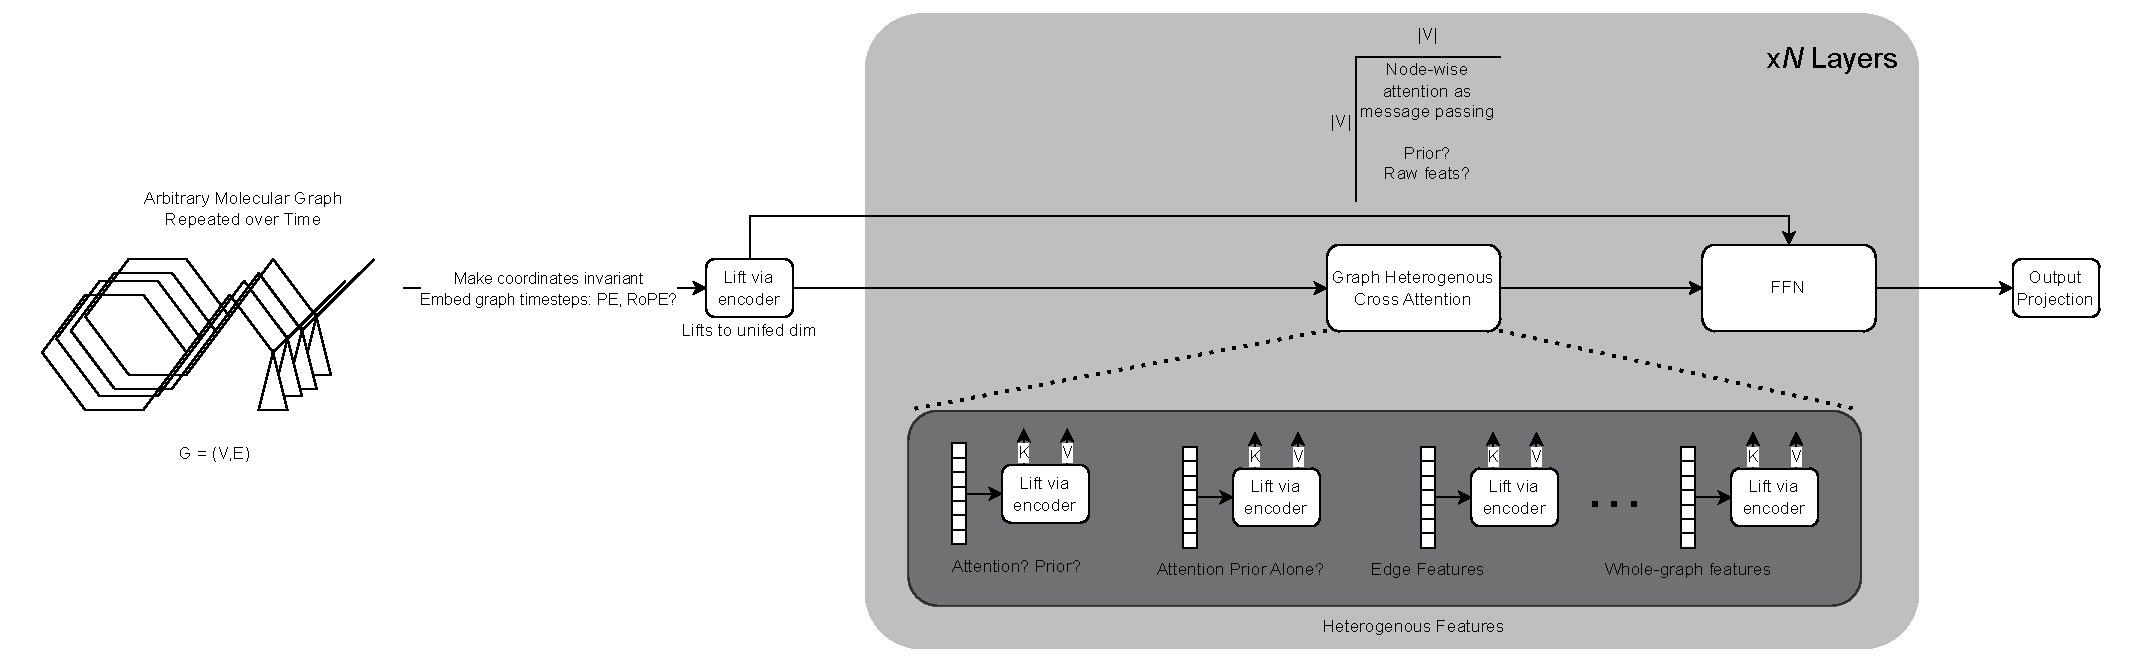
\includegraphics[width=1\linewidth]{Figures/GTNO-Page-1.drawio.pdf}
    \caption{\gls{gnot}-like architectire}
    \label{fig:gnot-arch}
\end{figure}

\subsubsection{EGNO-like Interleaving}
\label{sec:egno-based}
A generalisation of the \gls{egno} architecture to a graph transformer. We replace the explicit \gls{egnn} message passing with an attentional layer, and replace the Fourier temporal convolutions with a \gls{gnot}-like neural operator attention block.
\begin{figure}[h]
    \centering
    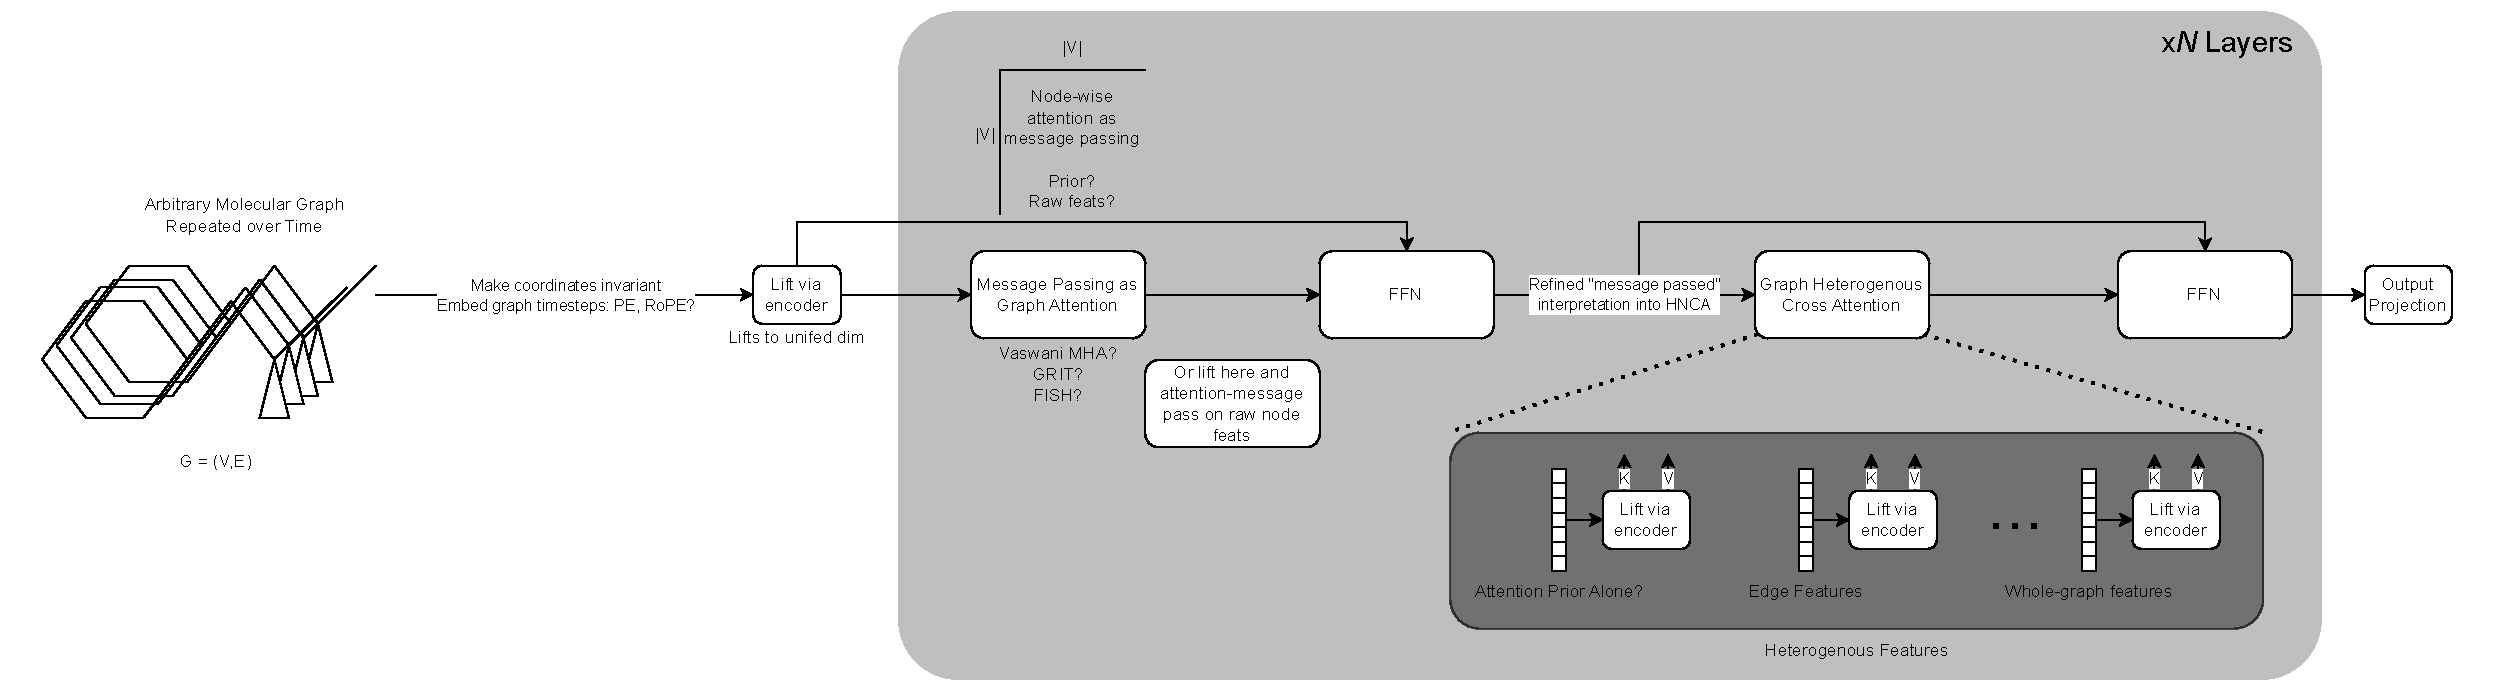
\includegraphics[width=1\linewidth]{Figures/GTNO-Page-2.drawio.pdf}
    \caption{\gls{egno}-like architecture}
    \label{fig:egno-arch}
\end{figure}

\section{Informal Architectural Overview}
\label{sec:headings}
\subsection{Attention Modalities}
\subsubsection{Standard attention as message passing}
For our \gls{egno}-based architecture \eqref{fig:egno-arch} we suggest placing a scaled-dot product attention block and \gls{ffn} before the G-HCNA block. This is akin to \textcite{xu_equivariant_2024}, where an explicit message passing graph neural network, \gls{egnn}, is placed before a neural operator block (\gls{fno}).

We anticipate this implict message-passing step would help refine graph node features before they are passed into subsequent blocks. A number of specific attentions are available, and may operate on the lifted or unlifted concatenated node feature vectors:
\begin{enumerate}
    \item Standard \gls{mha} \cite{vaswani_attention_2017}. The archetypal transformer attention with $\mathcal{O}(n^2)$ complexity.
    \item FiSH, a low rank attention mechanism wherein a subset of attention heads which learn linearly independent features are combined \cite{nguyen_improving_2022}. This is rare and not particularly advantageous for our task, but I list it as it was implemented in my previous paper \cite{thompson_amesformer_2024}.
    \item GRIT attention shows excellent performance in graph transformers and is specifically designed to achieve performance comparable to message-passing architectures without explicit \gls{gnn} blocks \cite{ma_graph_2023}.
\end{enumerate}

Our purely \gls{gnot}-derived architecture \eqref{fig:gnot-arch} does not include this separate attention-based message-passing step.

\subsubsection{Graph Heterogenous Normalised Cross-Attention}
Following \gls{gnot}, we propose Graph Heterogenous Normalised Cross-Attention (G-HNCA) \cite{hao_gnot_2023}. Let \( G_1, G_2, \dots, G_K \) represent \( K \) different graph representations \cite{hao_gnot_2023}. Each graph \( G_k \) contributes its own set of keys, queries, and values, denoted as:

\begin{itemize}
    \item Queries: \( \{q^{(k)}_i\}_{1 \leq i \leq N_k} \) from \( G_k \),
    \item Keys: \( \{k^{(k)}_i\}_{1 \leq i \leq M_k} \) from \( G_k \),
    \item Values: \( \{v^{(k)}_i\}_{1 \leq i \leq M_k} \) from \( G_k \),
\end{itemize}

where \( N_k \) and \( M_k \) denote the number of query and key-value pairs, respectively, for graph \( G_k \).

The heterogeneous attention \( z_t^{(k)} \) for a query \( q_t^{(k)} \) in graph \( G_k \) is computed as:

\[
z_t^{(k)} = \sum_{i=1}^{M_k} \frac{\exp\left(\frac{q_t^{(k)} \cdot k_i^{(k)}}{\tau}\right)}{\sum_{j=1}^{M_k} \exp\left(\frac{q_t^{(k)} \cdot k_j^{(k)}}{\tau}\right)} v_i^{(k)},
\]

where \( \tau \) is a temperature hyperparameter.

At this stage, we propose the following entries for the G-HCNA block:
\begin{enumerate}
    \item Attention priors alone could instead be introduced as their own $KV$ matrix, instead of as a prior in the attention block proper. This would be completely novel as far as I know. 
    \item Edge features, though this is dependent on the dataset makeup (i.e., MD17 does not contain edge features as the graphs are built according to a radius hyperparameter). It may be possible to embed an invariant Euclidean distance metric into the edges however.
    \item Whole-graph features. 
    \item It is also possible to include various graph rewirings with different curvature constants (e.g., Forman-Ricci), and compute attention across these. This may be a novel way to guard against oversmoothing and oversquashing simultaneously, assuming we could devise an appropriate gating mechanism for this task.
\end{enumerate}

\subsubsection{Attention Priors}
Following the terminology of \textcite{lin_survey_2021}, we describe data-dependent biases or prior information encoded into the attention blocks at their initialisation as \textit{attention priors}. This is additive with conventional (i.e., Xavier \cite{pmlr-v9-glorot10a}) initialisation methods. In most cases, attention biases in graph neural networks serve as positional encodings. We provide an inexhaustive list here:
\begin{enumerate}
    \item \textbf{Random-walk positional encodings} \cite{rampasek_recipe_2022} incorporate the stationary distribution of a random walk on the graph as a prior in the attention mechanism. Let \( P \) denote the random walk transition probability matrix, where \( P_{ij} \) represents the probability of transitioning from node \( i \) to node \( j \). The positional encoding for node \( i \) is derived from the \( i \)-th row of \( P^k \), where \( k \) is the number of steps in the random walk:
    \[
    \mathbf{p}_i = P^k[i, :]
    \]
    This encoding captures local graph structure and diffusion properties.

    \item \textbf{\gls{spd} positional encodings} \cite{chengxuan_transformers_2021} utilise the \( \text{SPD}(i, j) \) between two nodes \( i \) and \( j \) as a positional prior. The encoding is often represented as a kernel function \( f(\text{SPD}(i, j)) \), such as:
    \[
    \mathbf{p}_{ij} = \exp(-\beta \cdot \text{SPD}(i, j)),
    \]
    where \( \beta > 0 \) is a scaling parameter. The term "shortest-path distance" here refers to the minimum number of edges or weighted path length connecting two nodes in the graph. These encodings capture the global structure of the graph by integrating pairwise node distances into the attention mechanism.

    We have an existing Rust implementation of this \gls{spd} encoding via breadth-first search \href{https://github.com/luke-a-thompson/AmesFormer/tree/main/gnn-tools}{on GitHub} which shows excellent runtime performance up to large $|V|$.
\end{enumerate}

\subsection{Temporal Encodings}
\subsubsection{Transformer PE}
EGNO uses $\sin$ and $\cos$ embeddings akin to the positional encodings of transformers \cite{vaswani_attention_2017, xu_equivariant_2024}. These embeddings are necessary for their temporal convolutions, which convolve across the node-wise coordinates in Fourier space \cite{xu_equivariant_2024}.

\subsubsection{RoPE}
It would be novel to consider \gls{rope} embeddings, wherein the latent-space (query-key), representations of the input vectors are rotated according to their timestep. RoPE \cite{su_roformer_2023} shows better performance in \gls{nlp} and has been widely adopted \cite{grattafiori_llama_2024}. 

\subsubsection{Others}
There are a number of other approaches: FIRE, etc, but these are often specifically designed to exploit learned semantic interdependencies in natural language so are not as relevant.

\subsection{Evaluation}
Given the strong results of both \gls{egno} and \gls{gnot}, it is likely both would perform adequately for prediction on MD17. The specific tailoring of the \gls{egno} architecture with it's stacked message passing and neural operator blocks likely makes it the better choice. We anticipate it would be further enhanced by taking lessons from \gls{gnot} (which outperforms \gls{fno}, the basis of \gls{egno}).

\subsection{Datasets}
We have only investigated the MD17 molecular dynamics trajectory dataset thus far. We anticipate training on V2 of this dataset with reduced noise, as is recommended by the authors. This version was produced at a higher level of \gls{dft} theory.

Our model should also be applicable to \(n\)-body simulation and perhaps motion capture tasks.

\subsection{Other and Undeveloped Ideas}
\begin{enumerate}
    \item \textcite{delattre_efficient_2023} develop and efficient iterative approach for estimating the Lipschitz constant of \glspl{cnn}. They use this to perform Lipschitz regularisation, modestly boosting training stability. Where we to incorporate the Fourier-space temporal convolutions of \cite{xu_equivariant_2024} this could be advantageous as Lipschitz continuity bounds sensitivity to input variance which is especially important for high-dimensional \glspl{no}.
    \item Some research referenced in \textcite{le_mathematical_2024} suggests choosing activation functions which produce desirable Lipschitz constants. We believe we could extend this general thought to the automated tuning of parameterisable activation functions (e.g., parameterisable \gls{relu}) by Lipschitz estimate.
    \item We may be able to get empirical estimates of the Lipschitz constant of our \gls{no} via \cite{delattre_efficient_2023} and say something about its generalisation bounds \cite{le_mathematical_2024}.
    \item We could write this in a relatively novel Rust deep-learning framework
\end{enumerate}

\section{Conclusion}

\section*{Acknowledgments}

%Bibliography
\printbibliography
\printglossaries


\end{document}
